\section{Grundlagen}\label{sec:grundlagen}
In \cite{chesbrough2003} führt Henry W. Chesbrough erstmals die Begriffe \textit{Open} und
\textit{Closed Innovation} ein.
Mit diesen Begriffen bennent er zwei Paradigmen, welche den Innovationsprozess im Hinblick auf die
Interaktion mit der Umwelt des Unternehmens und dem Fluss von Wissen betrachtet.

Diese Seminararbeit behandelt vor allem die \textit{Closed Innovation}.
In den folgenden Unterkapiteln wird zunächst der Begriff \textit{Innovation} im Allgemeinen definiert.
Darufhin werden \textit{Closed Innovation} und grundlegend sein Gegenstück näher betrachtet.


\subsection{Innovation}\label{sec:grundlagen-inno}
Bevor die Begriffe \textit{Closed} und \textit{Open Innovation} näher betrachtet werden,
ist es notwendig den Begriff \textit{Innovation} an sich zu definieren.
Verschiedene Autoren definieren diesen Begriff auf unterschiedliche Arten.
In \cite[5]{hauschildt2016innovationsmanagement} ist eine Auswahl verschiedener Definitionen dargestellt.
Diese werden zusammengefasst zu der allgemeinen Aussage:
\begin{quote}
    \enquote{Innovationen sind qualitativ neuartige Produkte oder Verfahren,
    die sich gegenüber einem Vergleichszustand \enquote{merklich} [...] unterscheiden}
    \cite[4]{hauschildt2016innovationsmanagement}
\end{quote}

In \cite[9]{herzog2011} wird ein solches neuartiges Produkt oder Verfahen als \textit{Invention} bezeichnet und erst durch kommerzielle Verwertung zur \textit{Innovation}.
Die vorliegende Arbeit folgt dieser Definition.
Es gilt somit:
\begin{equation*}
    Innovation = Invention + kommerzielle~Verwertung
\end{equation*}

Hierbei ist zu beachten, dass der Begriff sich nicht nur auf Produkte bezieht, welche vermarktet werden,
sonder auch auf Prozesse, welche innerhalb der Produktion genutzt werden.

\subsection{Innovationsprozess}\label{sec:grundlagen-prozess}
\todo[inline]{Grob den Innovationsprozess beschreiben (Idee -> Ausarbeitung -> Vermarktung)}

\subsection{Closed Innovation}\label{sec:grundlagen-closed}

Das \textit{Closed Innovation}-Modell ist das vorherschende Innovationsmodell im 20. Jahrhundert.
Es spiegelt die damals vorherschende Wissensumgebung wider.
Unter Wissenschaftlern ist es verpönt ihre Fähigkeiten zu Nutzen um wirtschaftliche Probleme zu lösen.

Um dennoch Innovationen anzutreiben und so den kommerziellen Erfolg zu sichern,
sind Unternhemen gezwungen selbst in \ac{fe} zu investieren.
Da auch in anderen Unternehmen das notwendige Wissen noch nicht aufgebaut ist,
müssen Unternehmen innerhalb ihrer \ac{fe}-Organisation das gesamte Spektrum von den Grundlagen bis hin zum fertigen Produkt abdecken.
Voraussetzung hierfür ist die Akquise von talentierten Mitarbeitern.


\begin{figure}[ht!]
    \centering
    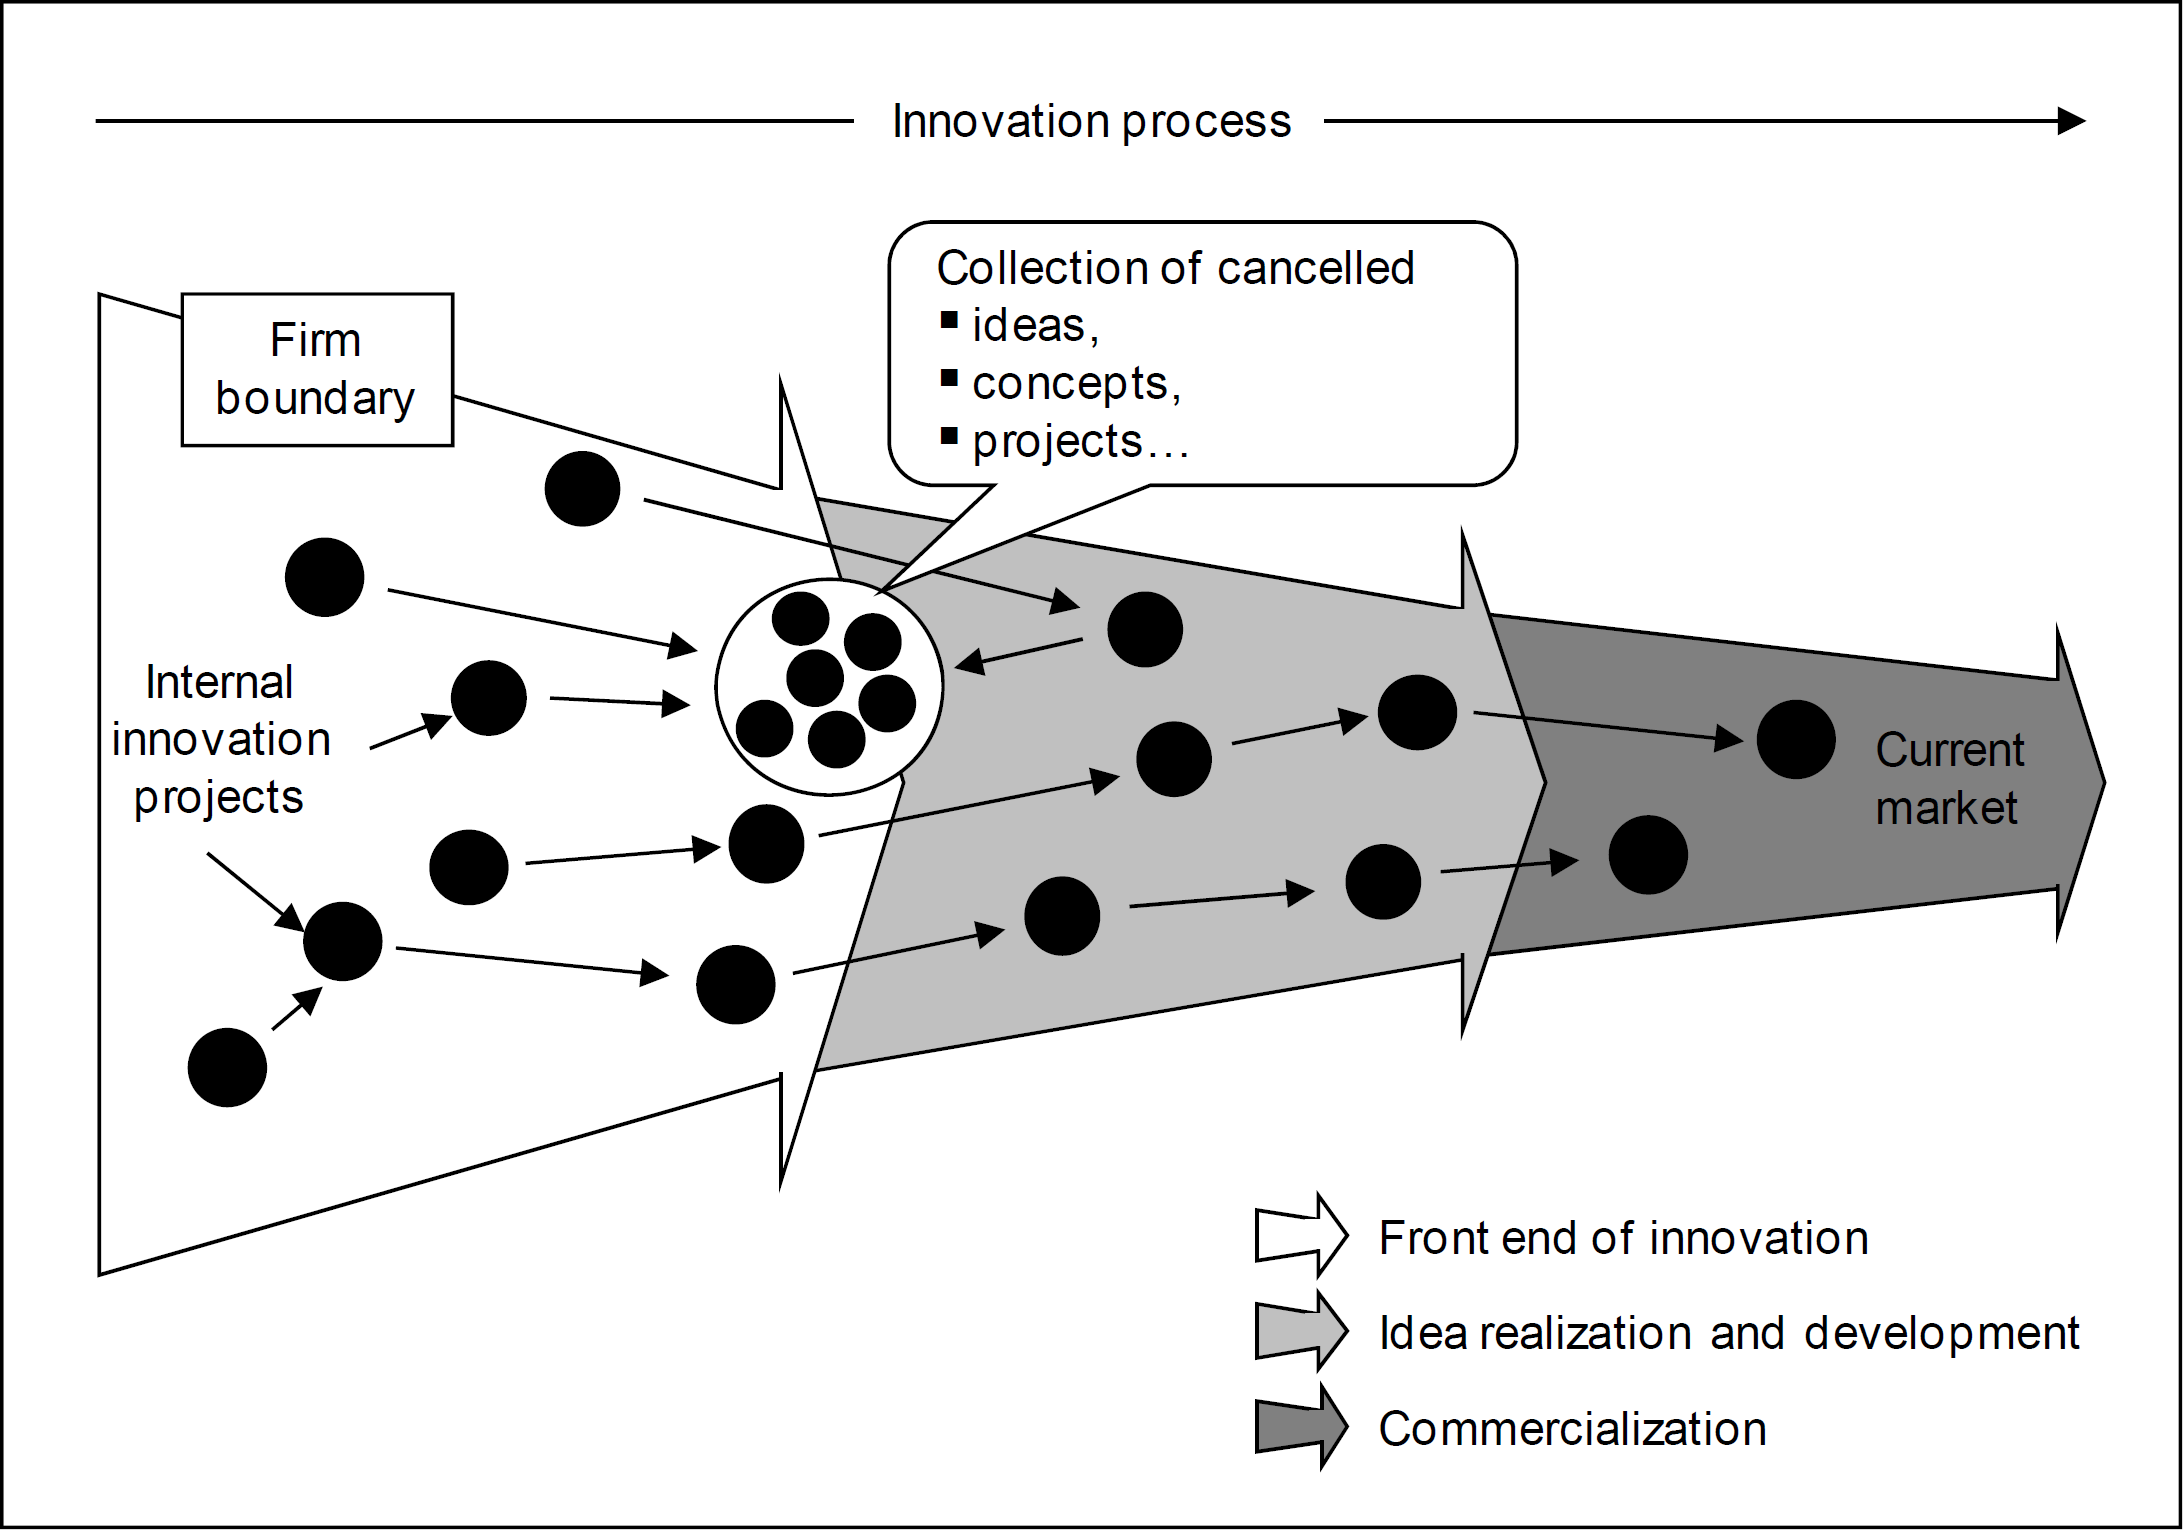
\includegraphics[width=1\textwidth]{ClosedInnovation}
    \caption{Closed Innovation Modell (aus \cite[20]{herzog2011})}
    \label{fig:closedInnovation}
\end{figure}

Altes Modell.
Damals muss.
Wegen: Forschung an Uni nicht Praxisnah
Fachkräfte müssen gebunden werden.
Forschung im Eigenen Unternehmen
Ideen nur von Innen
Ideen werden Umgesetzt oder Pausiert.

Keine neuen Märkte

\subsection{Open Innovation}\label{sec:grundlagen-open}

Neues Modell
Heute muss
Gründe: Wanderung von Fachkräften
Spezielle gebiete nich alleine erforschbar
Hohe Kosten
Uni forscht Praxisnah

Ideen kommen auch von Außen
Nicht umstzbare Ideen werden lizensiert oder outgesourced



\subsection{Kombination}\label{sec:grundlagen-kombi}

Beides lässt sich auch kombinieren